\documentclass[tikz,border=3mm]{standalone}
\usetikzlibrary{positioning, arrows.meta}

\begin{document}
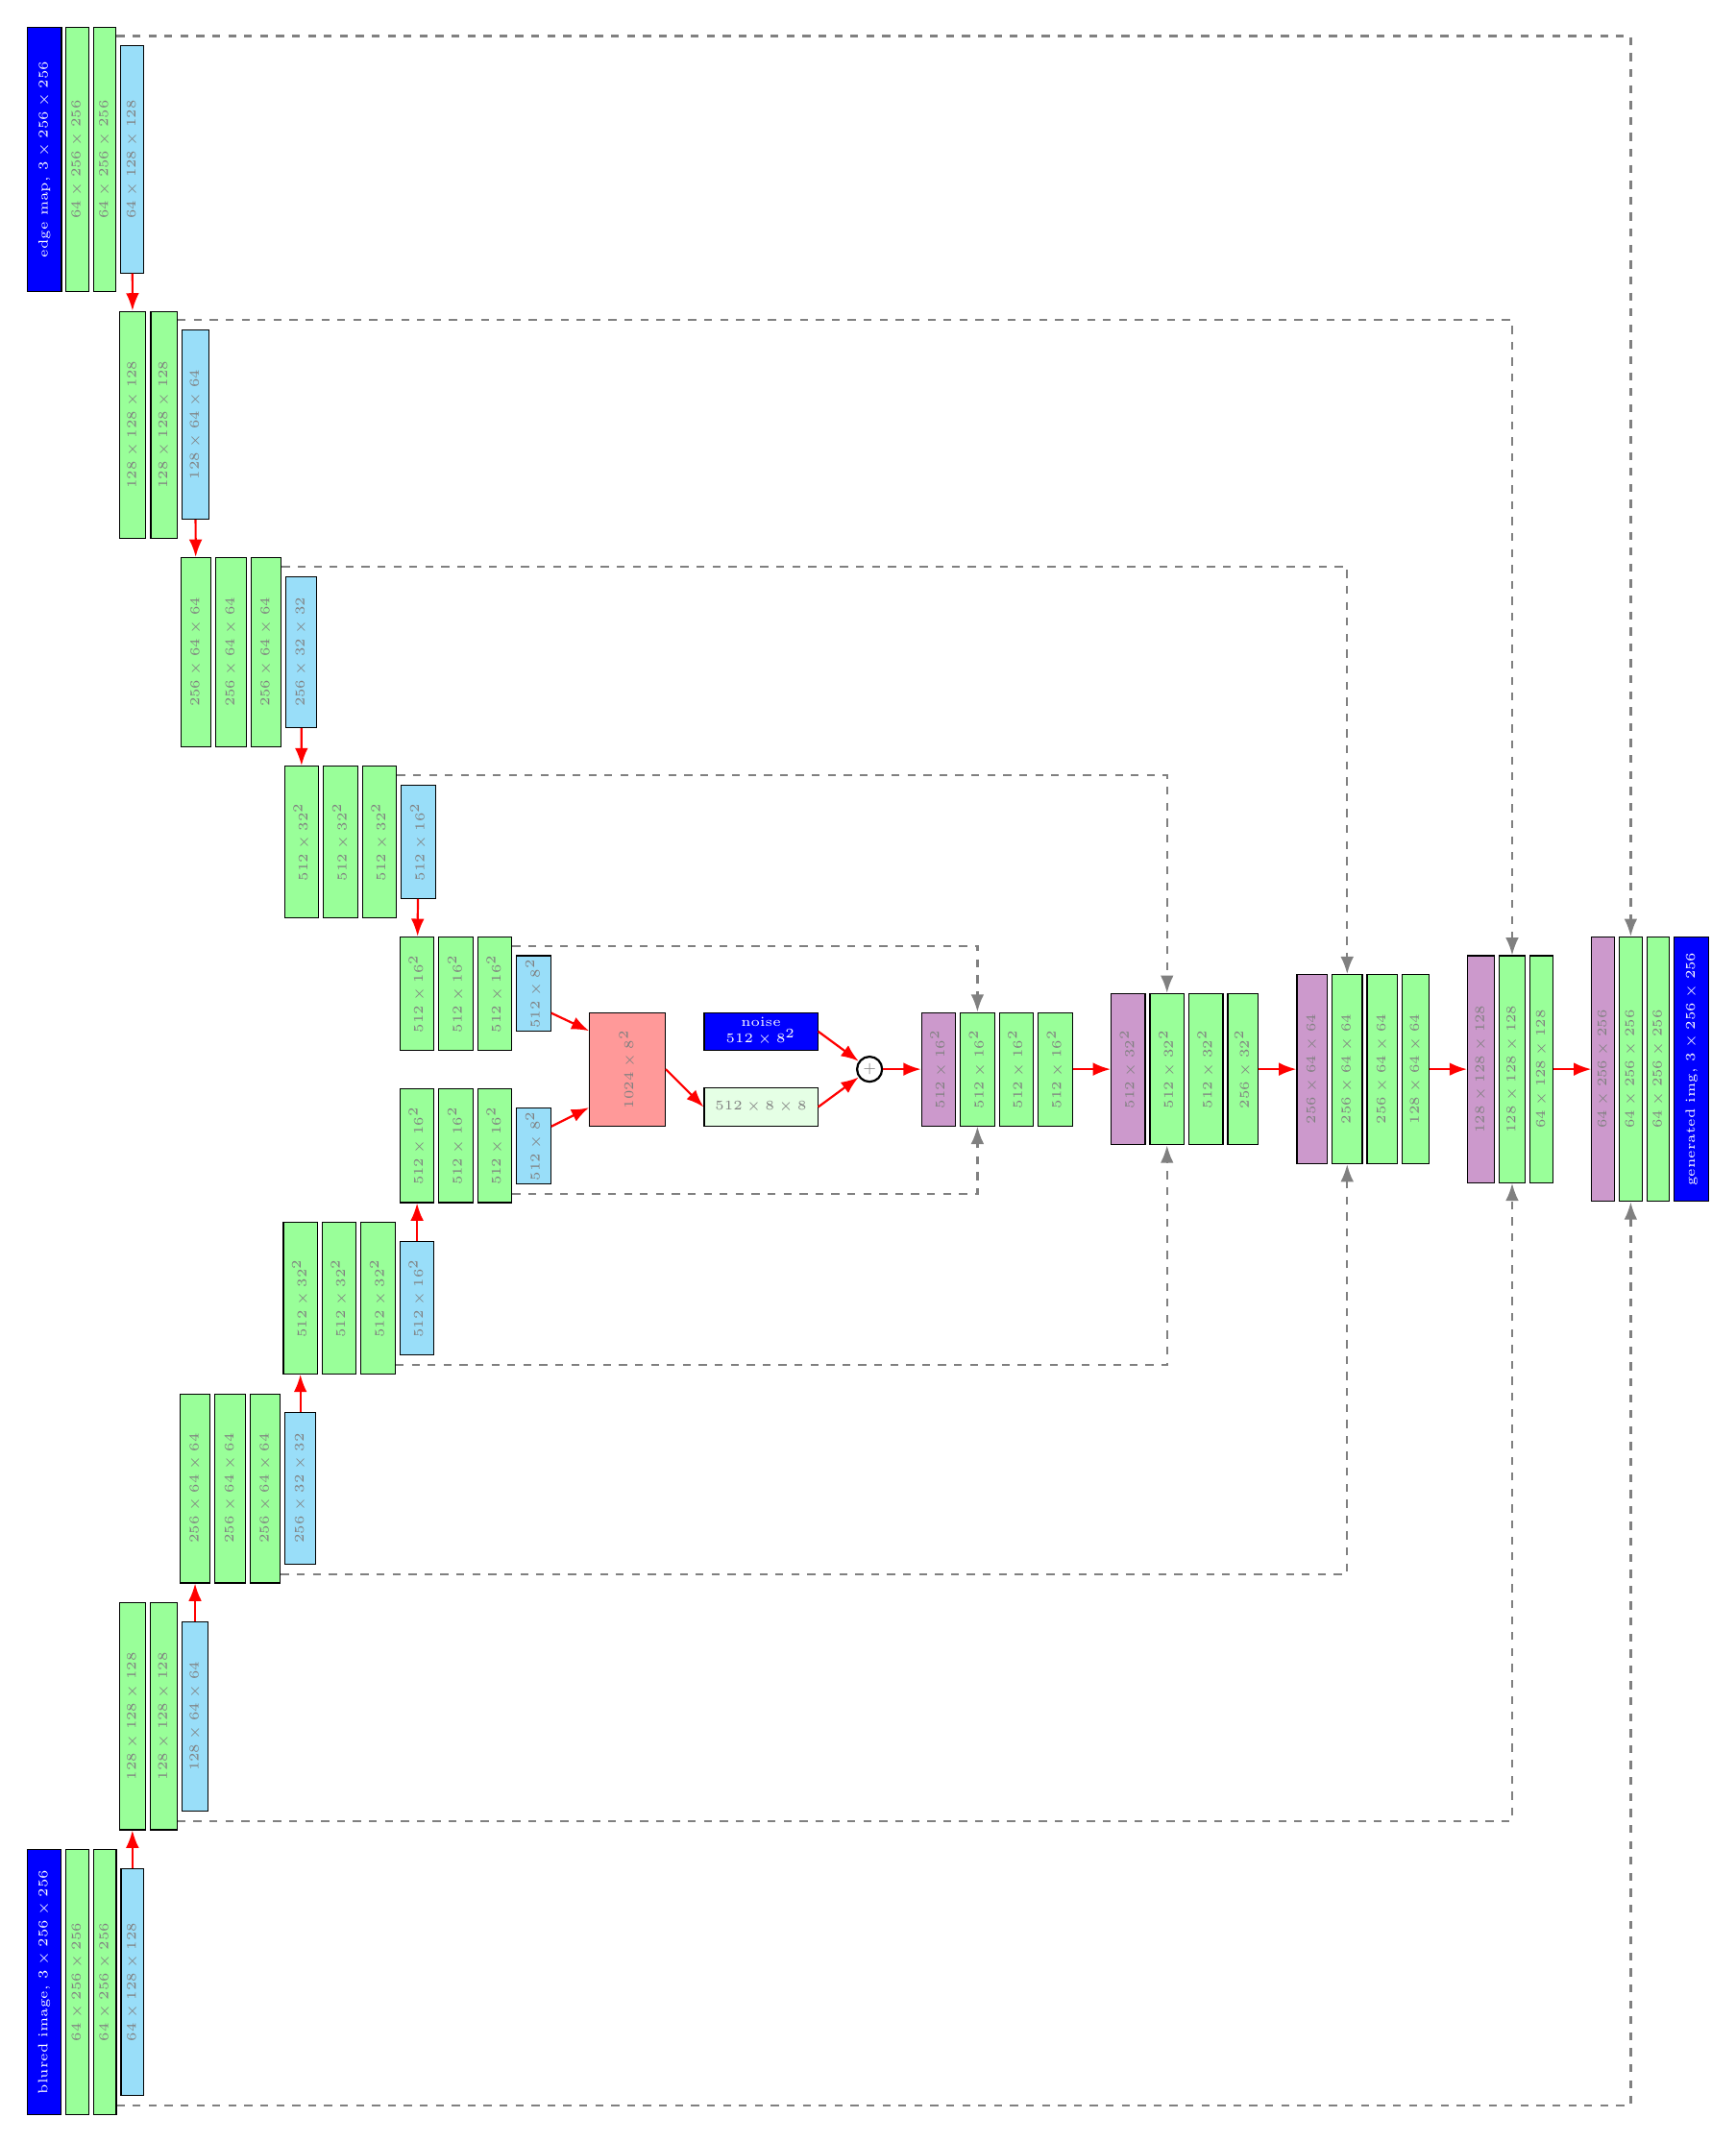
\begin{tikzpicture}[
    textLeft/.style         ={rotate=90,    anchor=south west,  align=left,     text=gray,  font=\tiny, inner xsep=0mm},
    textAbove/.style        ={rotate=0,     anchor=south,       align=left,     text=gray,  font=\tiny, inner xsep=0mm},
    textBelow/.style        ={rotate=0,     anchor=north east,  align=right,    text=gray,  font=\tiny, inner xsep=0mm},
    textInCent/.style       ={rotate=0,     anchor=east,        align=center,   text=gray,  font=\tiny, inner xsep=0mm},
    textInCentRot/.style    ={rotate=90,                        align=center,   text=gray,  font=\tiny, inner xsep=0mm},
    %
    image/.style        ={draw, fill=blue,      minimum width=0.45cm,   minimum height=3.5cm,   align=center},
    %
    conv_layer1/.style      ={draw, fill=green!40,  minimum width=0.3cm,    minimum height=3.5cm,   align=center},
    pool_layer1/.style      ={draw, fill=cyan!40,   minimum width=0.3cm,    minimum height=3cm,     align=center},
    unPool_layer1/.style    ={draw, fill=violet!40, minimum width=0.3cm,    minimum height=3.5cm,   align=center},
    deConv_layer1/.style    ={draw, fill=green!40,  minimum width=0.3cm,    minimum height=3.5cm,   align=center},
    %
    conv_layer2/.style      ={draw, fill=green!40,  minimum width=0.35cm,   minimum height=3cm,     align=center},
    pool_layer2/.style      ={draw, fill=cyan!40,   minimum width=0.35cm,   minimum height=2.5cm,   align=center},
    unPool_layer2/.style    ={draw, fill=violet!40, minimum width=0.35cm,    minimum height=3cm,     align=center},
    deConv_layer2_1/.style  ={draw, fill=green!40,  minimum width=0.35cm,    minimum height=3cm,     align=center},
    deConv_layer2_2/.style  ={draw, fill=green!40,  minimum width=0.3cm,   minimum height=3cm,     align=center},
    %
    conv_layer3/.style      ={draw, fill=green!40,  minimum width=0.4cm,    minimum height=2.5cm,   align=center},
    pool_layer3/.style      ={draw, fill=cyan!40,   minimum width=0.4cm,    minimum height=2cm,     align=center},
    unPool_layer3/.style=   {draw,  fill=violet!40, minimum width=0.4cm,   minimum height=2.5cm,   align=center},
    deConv_layer3_1/.style  ={draw, fill=green!40,  minimum width=0.4cm,   minimum height=2.5cm,   align=center},
    deConv_layer3_2/.style  ={draw, fill=green!40,  minimum width=0.35cm,   minimum height=2.5cm,   align=center},
    %
    conv_layer4/.style      ={draw, fill=green!40,  minimum width=0.45cm,   minimum height=2cm,     align=center},
    pool_layer4/.style      ={draw, fill=cyan!40,   minimum width=0.45cm,   minimum height=1.5cm,   align=center},
    unPool_layer4/.style    ={draw, fill=violet!40, minimum width=0.45cm,    minimum height=2cm,     align=center},
    deConv_layer4_1/.style  ={draw, fill=green!40,  minimum width=0.45cm,    minimum height=2cm,     align=center},
    deConv_layer4_2/.style  ={draw, fill=green!40,  minimum width=0.4cm,   minimum height=2cm,     align=center},
    %
    conv_layer5/.style      ={draw, fill=green!40,  minimum width=0.45cm,    minimum height=1.5cm,   align=center},
    pool_layer5/.style      ={draw, fill=cyan!40,   minimum width=0.45cm,    minimum height=1cm,     align=center},
    unPool_layer5/.style    ={draw, fill=violet!40, minimum width=0.45cm,    minimum height=1.5cm,   align=center},
    deConv_layer5/.style    ={draw, fill=green!40,  minimum width=0.45cm,   minimum height=1.5cm,   align=center},
    %
    cat_layer/.style    ={draw, fill=red!40,    minimum width=1cm,      minimum height=1.5cm,   align=center},
    1x1conv/.style      ={draw, fill=green!10,  minimum width=1.5cm,    minimum height=0.5cm,   align=center},
    noise_vector/.style ={draw, fill=blue,      minimum width=1.5cm,    minimum height=0.5cm,   align=center},
    sum/.style          ={draw, circle, thick, font=\tiny},
    %
    skiparrow/.style    ={draw, thick, dashed, gray, -Latex},
    arrow/.style        ={draw, thick, -Latex, color=red}
]

% Encoder path
\node[image] (input_map) {};
\node[textInCentRot, text=white] at (input_map) {edge map, $3 \times 256 \times 256$};

\node[conv_layer1, anchor=west] at ([xshift=0.275cm]input_map) (enc_1_1) {};
\node[textInCentRot] at (enc_1_1) {$64 \times 256 \times 256$};

\node[conv_layer1, anchor=west] at ([xshift=0.05cm]enc_1_1.east) (enc_1_2_map) {};
\node[textInCentRot] at (enc_1_2_map) {$64 \times 256 \times 256$};

\node[pool_layer1, anchor=west] at ([xshift=0.05cm]enc_1_2_map.east) (pool_1_map) {};
\node[textInCentRot] at (pool_1_map) {$64 \times 128 \times 128$};


\node[conv_layer2, anchor=west] at ([xshift=-0.175cm, yshift=-2cm]pool_1_map.south) (enc_2_1) {};
\node[textInCentRot] at (enc_2_1) {$128 \times 128 \times 128$};

\node[conv_layer2, anchor=west] at ([xshift=0.05cm]enc_2_1.east) (enc_2_2_map) {};
\node[textInCentRot] at (enc_2_2_map) {$128 \times 128 \times 128$};

\node[pool_layer2, anchor=west] at ([xshift=0.05cm]enc_2_2_map.east) (pool_2_map) {};
\node[textInCentRot] at (pool_2_map) {$128 \times 64 \times 64$};


\node[conv_layer3, anchor=west] at ([xshift=-0.2cm, yshift=-1.75cm]pool_2_map.south) (enc_3_1) {};
\node[textInCentRot] at (enc_3_1) {$256 \times 64 \times 64$};

\node[conv_layer3, anchor=west] at ([xshift=0.05cm]enc_3_1.east) (enc_3_2) {};
\node[textInCentRot] at (enc_3_2) {$256 \times 64 \times 64$};

\node[conv_layer3, anchor=west] at ([xshift=0.05cm]enc_3_2.east) (enc_3_3_map) {};
\node[textInCentRot] at (enc_3_3_map) {$256 \times 64 \times 64$};

\node[pool_layer3, anchor=west] at ([xshift=0.05cm]enc_3_3_map.east) (pool_3_map) {};
\node[textInCentRot] at (pool_3_map) {$256 \times 32 \times 32$};


\node[conv_layer4, anchor=west] at ([xshift=-0.225cm, yshift=-1.5cm]pool_3_map.south) (enc_4_1) {};
\node[textInCentRot] at (enc_4_1) {$512 \times 32^2$};

\node[conv_layer4, anchor=west] at ([xshift=0.05cm]enc_4_1.east) (enc_4_2) {};
\node[textInCentRot] at (enc_4_2) {$512 \times 32^2$};

\node[conv_layer4, anchor=west] at ([xshift=0.05cm]enc_4_2.east) (enc_4_3_map) {};
\node[textInCentRot] at (enc_4_3_map) {$512 \times 32^2$};

\node[pool_layer4, anchor=west] at ([xshift=0.05cm]enc_4_3_map.east) (pool_4_map) {};
\node[textInCentRot] at (pool_4_map) {$512 \times 16^2$};


\node[conv_layer5, anchor=west] at ([xshift=-0.25cm, yshift=-1.25cm]pool_4_map.south) (enc_5_1) {};
\node[textInCentRot] at (enc_5_1) {$512 \times 16^2$};

\node[conv_layer5, anchor=west] at ([xshift=0.05cm]enc_5_1.east) (enc_5_2) {};
\node[textInCentRot] at (enc_5_2) {$512 \times 16^2$};

\node[conv_layer5, anchor=west] at ([xshift=0.05cm]enc_5_2.east) (enc_5_3_map) {};
\node[textInCentRot] at (enc_5_3_map) {$512 \times 16^2$};

\node[pool_layer5, anchor=west] at ([xshift=0.05cm]enc_5_3_map.east) (pool_5_map) {};
\node[textInCentRot] at (pool_5_map) {$512 \times 8^2$};


\draw[arrow] (pool_1_map) -- (enc_2_1);
\draw[arrow] (pool_2_map) -- (enc_3_1);
\draw[arrow] (pool_3_map) -- (enc_4_1);
\draw[arrow] (pool_4_map) -- (enc_5_1);



\node[pool_layer5, anchor=north] at ([yshift=-1cm]pool_5_map.south) (pool_5_blur) {};
\node[textInCentRot] at (pool_5_blur) {$512 \times 8^2$};

\node[conv_layer5, anchor=east] at ([xshift=-0.05cm]pool_5_blur.west) (enc_5_3_blur) {};
\node[textInCentRot] at (enc_5_3_blur) {$512 \times 16^2$};

\node[conv_layer5, anchor=east] at ([xshift=-0.05cm]enc_5_3_blur.west) (enc_5_2) {};
\node[textInCentRot] at (enc_5_2) {$512 \times 16^2$};

\node[conv_layer5, anchor=east] at ([xshift=-0.05cm]enc_5_2.west) (enc_5_1) {};
\node[textInCentRot] at (enc_5_1) {$512 \times 16^2$};


\node[pool_layer4, anchor=north] at ([yshift=-0.5cm]enc_5_1.south) (pool_4_blur) {};
\node[textInCentRot] at (pool_4_blur) {$512 \times 16^2$};

\node[conv_layer4, anchor=east] at ([xshift=-0.05cm]pool_4_blur.west) (enc_4_3_blur) {};
\node[textInCentRot] at (enc_4_3_blur) {$512 \times 32^2$};

\node[conv_layer4, anchor=east] at ([xshift=-0.05cm]enc_4_3_blur.west) (enc_4_2) {};
\node[textInCentRot] at (enc_4_2) {$512 \times 32^2$};

\node[conv_layer4, anchor=east] at ([xshift=-0.05cm]enc_4_2.west) (enc_4_1) {};
\node[textInCentRot] at (enc_4_1) {$512 \times 32^2$};


\node[pool_layer3, anchor=north] at ([yshift=-0.5cm]enc_4_1.south) (pool_3_blur) {};
\node[textInCentRot] at (pool_3_blur) {$256 \times 32 \times 32$};

\node[conv_layer3, anchor=east] at ([xshift=-0.05cm]pool_3_blur.west) (enc_3_3_blur) {};
\node[textInCentRot] at (enc_3_3_blur) {$256 \times 64 \times 64$};

\node[conv_layer3, anchor=east] at ([xshift=-0.05cm]enc_3_3_blur.west) (enc_3_2) {};
\node[textInCentRot] at (enc_3_2) {$256 \times 64 \times 64$};

\node[conv_layer3, anchor=east] at ([xshift=-0.05cm]enc_3_2.west) (enc_3_1) {};
\node[textInCentRot] at (enc_3_1) {$256 \times 64 \times 64$};


\node[pool_layer2, anchor=north] at ([yshift=-0.5cm]enc_3_1.south) (pool_2_blur) {};
\node[textInCentRot] at (pool_2_blur) {$128 \times 64 \times 64$};

\node[conv_layer2, anchor=east] at ([xshift=-0.05cm]pool_2_blur.west) (enc_2_2_blur) {};
\node[textInCentRot] at (enc_2_2_blur) {$128 \times 128 \times 128$};

\node[conv_layer2, anchor=east] at ([xshift=-0.05cm]enc_2_2_blur.west) (enc_2_1) {};
\node[textInCentRot] at (enc_2_1) {$128 \times 128 \times 128$};


\node[pool_layer1, anchor=north] at ([yshift=-0.5cm]enc_2_1.south) (pool_1_blur) {};
\node[textInCentRot] at (pool_1_blur) {$64 \times 128 \times 128$};

\node[conv_layer1, anchor=east] at ([xshift=-0.05cm]pool_1_blur.west) (enc_1_2_blur) {};
\node[textInCentRot] at (enc_1_2_blur) {$64 \times 256 \times 256$};

\node[conv_layer1, anchor=east] at ([xshift=-0.05cm]enc_1_2_blur.west) (enc_1_1) {};
\node[textInCentRot] at (enc_1_1) {$64 \times 256 \times 256$};

\node[image, anchor=east] at([xshift=-0.05cm]enc_1_1.west) (input_blur) {};
\node[textInCentRot, text=white] at (input_blur) {blured image, $3 \times 256 \times 256$};


\draw[arrow] (pool_1_blur) -- (enc_2_1);
\draw[arrow] (pool_2_blur) -- (enc_3_1);
\draw[arrow] (pool_3_blur) -- (enc_4_1);
\draw[arrow] (pool_4_blur) -- (enc_5_1);



\node[cat_layer, anchor=west] at ([xshift=0.5cm, yshift=-1cm]pool_5_map.east) (latent) {};
\node[textInCentRot, anchor=center] at (latent) {$1024 \times 8^2$};


\draw[arrow] ([yshift=0.25cm]pool_5_map.south east) -- ([yshift=-0.25cm]latent.north west);
\draw[arrow] ([yshift=-0.25cm]pool_5_blur.north east) -- ([yshift=0.25cm]latent.south west);



\node[1x1conv, anchor=south west] at ([xshift=0.5cm]latent.south east) (conv1x1_latSpace) {};
\node[textInCent, anchor=center] at (conv1x1_latSpace) {$512 \times 8 \times 8$};

\node[noise_vector, anchor=north west] at ([xshift=0.5cm]latent.north east) (noise_conv_1) {};
\node[textInCent, text=white, anchor=center] at (noise_conv_1) {noise\\$512 \times 8^2$};

\node[sum, anchor=west] at ([xshift=0.5cm, yshift=0.5cm]conv1x1_latSpace.east) (sum_node) {};
\node[textInCent, anchor=center] at (sum_node) {$+$};


\draw[arrow] (latent.east) -- (conv1x1_latSpace.west);
\draw[arrow] (noise_conv_1.east) -- (sum_node);
\draw[arrow] (conv1x1_latSpace.east) -- (sum_node);



\node[unPool_layer5, anchor=west] at ([xshift=0.5cm]sum_node.east) (unPool_5) {};
\node[textInCentRot] at (unPool_5) {$512 \times 16^2$};

\node[deConv_layer5, anchor=west] at ([xshift=0.05cm]unPool_5.east) (dec_5_1) {};
\node[textInCentRot] at (dec_5_1) {$512 \times 16^2$};

\node[deConv_layer5, anchor=west] at ([xshift=0.05cm]dec_5_1.east) (dec_5_2) {};
\node[textInCentRot] at (dec_5_2) {$512 \times 16^2$};

\node[deConv_layer5, anchor=west] at ([xshift=0.05cm]dec_5_2.east) (dec_5_3) {};
\node[textInCentRot] at (dec_5_3) {$512 \times 16^2$};


\node[unPool_layer4, anchor=west] at ([xshift=0.5cm]dec_5_3.east) (unPool_4) {};
\node[textInCentRot] at (unPool_4) {$512 \times 32^2$};

\node[deConv_layer4_1, anchor=west] at ([xshift=0.05cm]unPool_4.east) (dec_4_1) {};
\node[textInCentRot] at (dec_4_1) {$512 \times 32^2$};

\node[deConv_layer4_1, anchor=west] at ([xshift=0.05cm]dec_4_1.east) (dec_4_2) {};
\node[textInCentRot] at (dec_4_2) {$512 \times 32^2$};

\node[deConv_layer4_2, anchor=west] at ([xshift=0.05cm]dec_4_2.east) (dec_4_3) {};
\node[textInCentRot] at (dec_4_3) {$256 \times 32^2$};


\node[unPool_layer3, anchor=west] at ([xshift=0.5cm]dec_4_3.east) (unPool_3) {};
\node[textInCentRot] at (unPool_3) {$256 \times 64 \times 64$};

\node[deConv_layer3_1, anchor=west] at ([xshift=0.05cm]unPool_3.east) (dec_3_1) {};
\node[textInCentRot] at (dec_3_1) {$256 \times 64 \times 64$};

\node[deConv_layer3_1, anchor=west] at ([xshift=0.05cm]dec_3_1.east) (dec_3_2) {};
\node[textInCentRot] at (dec_3_2) {$256 \times 64 \times 64$};

\node[deConv_layer3_2, anchor=west] at ([xshift=0.05cm]dec_3_2.east) (dec_3_3) {};
\node[textInCentRot] at (dec_3_3) {$128 \times 64 \times 64$};


\node[unPool_layer2, anchor=west] at ([xshift=0.5cm]dec_3_3.east) (unPool_2) {};
\node[textInCentRot] at (unPool_2) {$128 \times 128 \times 128$};

\node[deConv_layer2_1, anchor=west] at ([xshift=0.05cm]unPool_2.east) (dec_2_1) {};
\node[textInCentRot] at (dec_2_1) {$128 \times 128 \times 128$};

\node[deConv_layer2_2, anchor=west] at ([xshift=0.05cm]dec_2_1.east) (dec_2_2) {};
\node[textInCentRot] at (dec_2_2) {$64 \times 128 \times 128$};


\node[unPool_layer1, anchor=west] at ([xshift=0.5cm]dec_2_2.east) (unPool_1) {};
\node[textInCentRot] at (unPool_1) {$64 \times 256 \times 256$};

\node[deConv_layer1, anchor=west] at ([xshift=0.05cm]unPool_1.east) (dec_1_1) {};
\node[textInCentRot] at (dec_1_1) {$64 \times 256 \times 256$};

\node[deConv_layer1, anchor=west] at ([xshift=0.05cm]dec_1_1.east) (dec_1_2) {};
\node[textInCentRot] at (dec_1_2) {$64 \times 256 \times 256$};

\node[image, anchor=west] (gen_img) at ([xshift=0.05cm]dec_1_2.east) {};
\node[textInCentRot, text=white] at (gen_img) {generated img, $3 \times 256 \times 256$};


\draw[arrow] (sum_node) -- (unPool_5);
\draw[arrow] (dec_5_3) -- (unPool_4);
\draw[arrow] (dec_4_3) -- (unPool_3);
\draw[arrow] (dec_3_3) -- (unPool_2);
\draw[arrow] (dec_2_2) -- (unPool_1);



\draw[skiparrow] ([yshift=-0.125cm]enc_5_3_map.north east) -| (dec_5_1.north);
\draw[skiparrow] ([yshift=-0.125cm]enc_4_3_map.north east) -| (dec_4_1.north);
\draw[skiparrow] ([yshift=-0.125cm]enc_3_3_map.north east) -| (dec_3_1.north);
\draw[skiparrow] ([yshift=-0.125cm]enc_2_2_map.north east) -| (dec_2_1.north);
\draw[skiparrow] ([yshift=-0.125cm]enc_1_2_map.north east) -| (dec_1_1.north);

\draw[skiparrow] ([yshift=0.125cm]enc_5_3_blur.south east) -| (dec_5_1.south);
\draw[skiparrow] ([yshift=0.125cm]enc_4_3_blur.south east) -| (dec_4_1.south);
\draw[skiparrow] ([yshift=0.125cm]enc_3_3_blur.south east) -| (dec_3_1.south);
\draw[skiparrow] ([yshift=0.125cm]enc_2_2_blur.south east) -| (dec_2_1.south);
\draw[skiparrow] ([yshift=0.125cm]enc_1_2_blur.south east) -| (dec_1_1.south);




\end{tikzpicture}
\end{document}







% \documentclass[tikz,border=3mm]{standalone}
% \usetikzlibrary{positioning, arrows.meta}

% \begin{document}
% \begin{tikzpicture}[
%     textLeft/.style         ={rotate=90,    anchor=south west,  align=left,     text=gray,  font=\scriptsize, inner xsep=0mm},
%     textAbove/.style        ={rotate=0,     anchor=south,       align=left,     text=gray,  font=\scriptsize, inner xsep=0mm},
%     textBelow/.style        ={rotate=0,     anchor=north east,  align=right,    text=gray,  font=\scriptsize, inner xsep=0mm},
%     textInCent/.style       ={rotate=0,     anchor=east,        align=center,   text=gray,  font=\scriptsize, inner xsep=0mm},
%     textInCentRot/.style    ={rotate=90,                        align=center,   text=gray,  font=\scriptsize, inner xsep=0mm},
%     image/.style        ={draw, fill=blue,      minimum width=0.45cm,   minimum height=3.5cm,   align=center,   anchor=west},
%     conv_layer1/.style  ={draw, fill=green!40,  minimum width=0.3cm,    minimum height=3.5cm,   align=center,   anchor=west},
%     pool_layer1/.style  ={draw, fill=cyan!40,   minimum width=0.3cm,    minimum height=3.5cm,   align=center,   anchor=west},
%     conv_layer2/.style  ={draw, fill=green!40,  minimum width=0.35cm,   minimum height=3cm,     align=center,   anchor=west},
%     pool_layer2/.style  ={draw, fill=cyan!40,   minimum width=0.35cm,   minimum height=3cm,     align=center,   anchor=west},
%     conv_layer3/.style  ={draw, fill=green!40,  minimum width=0.4cm,    minimum height=2.5cm,   align=center,   anchor=west},
%     pool_layer3/.style  ={draw, fill=cyan!40,   minimum width=0.4cm,    minimum height=2.5cm,   align=center,   anchor=west},
%     conv_layer4/.style  ={draw, fill=green!40,  minimum width=0.45cm,   minimum height=2cm,     align=center,   anchor=west},
%     pool_layer4/.style  ={draw, fill=cyan!40,   minimum width=0.45cm,   minimum height=2cm,     align=center,   anchor=west},
%     conv_layer5/.style  ={draw, fill=green!40,  minimum width=0.5cm,    minimum height=1.5cm,   align=center,   anchor=west},
%     pool_layer5/.style  ={draw, fill=cyan!40,   minimum width=0.5cm,    minimum height=1.5cm,   align=center,   anchor=west},
%     latent_space/.style ={draw, fill=red!40,    minimum width=4.35cm,   minimum height=1cm,     align=center,   anchor=north east},
%     1x1conv/.style      ={draw, fill=green!10,  minimum width=1.5cm,    minimum height=0.5cm,   align=center,   anchor=west},
%     noise_conv/.style   ={draw, fill=gray!40,   minimum width=0.5cm,    minimum height=1.5cm,   align=center,   anchor=west},
%     sum/.style          ={draw, circle, thick, minimum size=0.5cm, font= \scriptsize},
%     upconv/.style       ={draw, fill=yellow!40, minimum width=1.2cm,    minimum height=1cm,     align=center,   anchor=west},
%     skiparrow/.style={draw, thick, dashed, red, -Latex},
%     arrow/.style={draw, thick, -Latex},
%     layerlabel/.style={font=\small}
% ]

% % Encoder path
% \node[image] (input_map) {};
% \node[textInCentRot, text=white] at (input_map) {edge map, $3 \times 256 \times 256$};

% \node[conv_layer1] at ([xshift=0.275cm]input_map) (enc_1_1) {};
% \node[textInCentRot] at (enc_1_1) {$64 \times 256 \times 256$};

% \node[conv_layer1] at ([xshift=0.05cm]enc_1_1.east) (enc_1_2) {};
% \node[textInCentRot] at (enc_1_2) {$64 \times 256 \times 256$};

% \node[pool_layer1] at ([xshift=0.05cm]enc_1_2.east) (pool_1) {};
% \node[textInCentRot] at (pool_1) {$64 \times 128 \times 128$};


% \node[conv_layer2] at ([xshift=-0.175cm, yshift=-2cm]pool_1.south) (enc_2_1) {};
% \node[textInCentRot] at (enc_2_1) {$128 \times 128 \times 128$};

% \node[conv_layer2] at ([xshift=0.05cm]enc_2_1.east) (enc_2_2) {};
% \node[textInCentRot] at (enc_2_2) {$128 \times 128 \times 128$};

% \node[pool_layer2] at ([xshift=0.05cm]enc_2_2.east) (pool_2) {};
% \node[textInCentRot] at (pool_2) {$128 \times 64 \times 64$};


% \node[conv_layer3] at ([xshift=-0.2cm, yshift=-1.75cm]pool_2.south) (enc_3_1) {};
% \node[textInCentRot] at (enc_3_1) {$256 \times 64 \times 64$};

% \node[conv_layer3] at ([xshift=0.05cm]enc_3_1.east) (enc_3_2) {};
% \node[textInCentRot] at (enc_3_2) {$256 \times 64 \times 64$};

% \node[conv_layer3] at ([xshift=0.05cm]enc_3_2.east) (enc_3_3) {};
% \node[textInCentRot] at (enc_3_3) {$256 \times 64 \times 64$};

% \node[pool_layer3] at ([xshift=0.05cm]enc_3_3.east) (pool_3) {};
% \node[textInCentRot] at (pool_3) {$256 \times 32 \times 32$};


% \node[conv_layer4] at ([xshift=-0.225cm, yshift=-1.5cm]pool_3.south) (enc_4_1) {};
% \node[textInCentRot] at (enc_4_1) {$512 \times 32^2$};

% \node[conv_layer4] at ([xshift=0.05cm]enc_4_1.east) (enc_4_2) {};
% \node[textInCentRot] at (enc_4_2) {$512 \times 32^2$};

% \node[conv_layer4] at ([xshift=0.05cm]enc_4_2.east) (enc_4_3) {};
% \node[textInCentRot] at (enc_4_3) {$512 \times 32^2$};

% \node[pool_layer4] at ([xshift=0.05cm]enc_4_3.east) (pool_4) {};
% \node[textInCentRot] at (pool_4) {$512 \times 16^2$};


% \node[conv_layer5] at ([xshift=-0.25cm, yshift=-1.25cm]pool_4.south) (enc_5_1) {};
% \node[textInCentRot] at (enc_5_1) {$512 \times 16^2$};

% \node[conv_layer5] at ([xshift=0.05cm]enc_5_1.east) (enc_5_2) {};
% \node[textInCentRot] at (enc_5_2) {$512 \times 16^2$};

% \node[conv_layer5] at ([xshift=0.05cm]enc_5_2.east) (enc_5_3) {};
% \node[textInCentRot] at (enc_5_3) {$512 \times 16^2$};

% \node[pool_layer5] at ([xshift=0.05cm]enc_5_3.east) (pool_5_map) {};
% \node[textInCentRot] at (pool_5_map) {$512 \times 8^2$};


% \draw[arrow, color=red] (pool_1) -- (enc_2_1);
% \draw[arrow, color=red] (pool_2) -- (enc_3_1);
% \draw[arrow, color=red] (pool_3) -- (enc_4_1);
% \draw[arrow, color=red] (pool_4) -- (enc_5_1);



% \node[image] at([yshift=7cm]pool_3) (input_blur) {};
% \node[textInCentRot, text=white] at (input_blur) {blured image, $3 \times 256 \times 256$};

% \node[conv_layer1] at ([xshift=0.275cm]input_blur) (enc_1_1) {};
% \node[textInCentRot] at (enc_1_1) {$64 \times 256 \times 256$};

% \node[conv_layer1] at ([xshift=0.05cm]enc_1_1.east) (enc_1_2) {};
% \node[textInCentRot] at (enc_1_2) {$64 \times 256 \times 256$};

% \node[pool_layer1] at ([xshift=0.05cm]enc_1_2.east) (pool_1) {};
% \node[textInCentRot] at (pool_1) {$64 \times 128 \times 128$};


% \node[conv_layer2] at ([xshift=-0.175cm, yshift=-2cm]pool_1.south) (enc_2_1) {};
% \node[textInCentRot] at (enc_2_1) {$128 \times 128 \times 128$};

% \node[conv_layer2] at ([xshift=0.05cm]enc_2_1.east) (enc_2_2) {};
% \node[textInCentRot] at (enc_2_2) {$128 \times 128 \times 128$};

% \node[pool_layer2] at ([xshift=0.05cm]enc_2_2.east) (pool_2) {};
% \node[textInCentRot] at (pool_2) {$128 \times 64 \times 64$};


% \node[conv_layer3] at ([yshift=-3.25cm]pool_2) (enc_3_1) {};
% \node[textInCentRot] at (enc_3_1) {$256 \times 64 \times 64$};

% \node[conv_layer3] at ([xshift=0.05cm]enc_3_1.east) (enc_3_2) {};
% \node[textInCentRot] at (enc_3_2) {$256 \times 64 \times 64$};

% \node[conv_layer3] at ([xshift=0.05cm]enc_3_2.east) (enc_3_3) {};
% \node[textInCentRot] at (enc_3_3) {$256 \times 64 \times 64$};

% \node[pool_layer3] at ([xshift=0.05cm]enc_3_3.east) (pool_3) {};
% \node[textInCentRot] at (pool_3) {$256 \times 32 \times 32$};


% \node[conv_layer4] at ([xshift=-0.225cm, yshift=-1.5cm]pool_3.south) (enc_4_1) {};
% \node[textInCentRot] at (enc_4_1) {$512 \times 32^2$};

% \node[conv_layer4] at ([xshift=0.05cm]enc_4_1.east) (enc_4_2) {};
% \node[textInCentRot] at (enc_4_2) {$512 \times 32^2$};

% \node[conv_layer4] at ([xshift=0.05cm]enc_4_2.east) (enc_4_3) {};
% \node[textInCentRot] at (enc_4_3) {$512 \times 32^2$};

% \node[pool_layer4] at ([xshift=0.05cm]enc_4_3.east) (pool_4) {};
% \node[textInCentRot] at (pool_4) {$512 \times 16^2$};


% \node[conv_layer5] at ([xshift=-0.225cm, yshift=-1.25cm]pool_4.south) (enc_5_1) {};
% \node[textInCentRot] at (enc_5_1) {$512 \times 16^2$};

% \node[conv_layer5] at ([xshift=0.05cm]enc_5_1.east) (enc_5_2) {};
% \node[textInCentRot] at (enc_5_2) {$512 \times 16^2$};

% \node[conv_layer5] at ([xshift=0.05cm]enc_5_2.east) (enc_5_3) {};
% \node[textInCentRot] at (enc_5_3) {$512 \times 16^2$};

% \node[pool_layer5] at ([xshift=0.05cm]enc_5_3.east) (pool_5_blur) {};
% \node[textInCentRot] at (pool_5_blur) {$512 \times 8^2$};


% \draw[arrow, color=red] (pool_1) -- (enc_2_1);
% \draw[arrow, color=red] (pool_2) -- (enc_3_1);
% \draw[arrow, color=red] (pool_3) -- (enc_4_1);
% \draw[arrow, color=red] (pool_4) -- (enc_5_1);



% \node[latent_space] at ([yshift=-0.5cm]pool_5_blur.south east) (latent) {};
% \node[textInCent, anchor=center] at (latent) {$1024 \times 8 \times 8$};


% \node[1x1conv] at ([xshift=0.5cm]latent.east) (conv1x1_latSpace) {};
% \node[textInCent, anchor=center] at (conv1x1_latSpace) {$512 \times 8 \times 8$};


% \draw[arrow, color=red] 
%     (pool_5_map.south) -- ++(0,-0.5cm);
% \draw[arrow, color=red] 
%     (pool_5_blur.south) -- ++(0,-0.5cm);
% \draw[arrow, color=red] 
%     (latent.east) -- (conv1x1_latSpace.west);

% \node[sum] at ([xshift=0.75cm]conv1x1_latSpace.east) (sum_node) {};
% \node[textInCent, anchor=center] at (sum_node) {$+$};

% \node[noise_conv, anchor=south] at ([yshift=1cm]sum_node) (noise_conv_1) {};
% \node[textInCentRot] at (noise_conv_1) {$512 \times 8^2$};

% \node[image, anchor=south] at ([yshift=1.25cm]noise_conv_1) (noise_vector) {};
% \node[textInCentRot, text=white] at (noise_vector) {noise, $100 \times 1 \times 1$};

% \draw[arrow, color=red] (noise_vector) -- (noise_conv_1);
% \draw[arrow, color=red] (noise_conv_1) -- (sum_node);
% \draw[arrow, color=red] (conv1x1_latSpace) -- (sum_node);




% \end{tikzpicture}
% \end{document}